\documentclass[11pt]{amsart}
\usepackage[margin=1in]{geometry}                % See geometry.pdf to learn the layout options. There are lots.
\geometry{letterpaper}                   % ... or a4paper or a5paper or ... 
%\geometry{landscape}                % Activate for for rotated page geometry
%\usepackage[parfill]{parskip}    % Activate to begin paragraphs with an empty line rather than an indent
\usepackage{graphicx}
\usepackage{amssymb}
\usepackage{epstopdf}
\usepackage{wrapfig}
\usepackage[margin=10pt,font=small,labelfont=bf,
               labelsep=colon]{caption}

\DeclareGraphicsRule{.tif}{png}{.png}{`convert #1 `dirname #1`/`basename #1 .tif`.png}



\title{ALDEx2: ANOVA-Like Differential Expression tool for compositional data}
\author{Andrew Fernandes, Jean Macklaim, Gregory Gloor}
\date{\today}                                           % Activate to display a given date or no date

\begin{document}
\maketitle

\section{Introduction}
This guide provides an overview of the R package ALDEx version 2 (ALDEx2) for differential expression analysis of proportional data. The package was developed specifically for multiple-organism RNA-Seq data generated by high-throughput sequencing platforms (meta-RNA-Seq), but testing showed that it performed very well with traditional RNA-Seq datasets, 16S rRNA variable region sequencing and selective growth-type (SELEX) experiments. In principle, the analysis method should be applicable to nearly any type of data that is generated by high-throughput sequencing that generates tables of feature or feature counts for each sample: in addition to the examples outlined above this would include  ChIP-Seq or metagenome sequencing. See the following examples for application on these types of problems.

The ALDEx2 package is suitable for comparison of samples between two conditions where there are at least three biological replicates per condition. If there are only two replicates in one condition the user is advised to use ALDEx version 1. Both ALDEx and ALDEx2 use the same underlying method of estimating per-feature variation in each sample and the same method of transforming the data into relative abundance values. Per-feature technical variation within each sample is estimated using the Dirichlet distribution. This distribution maintains the proportional nature of the data. Both versions of ALDEx use the centred log-ratio (clr) transformation that ensures the data are scale invariant and sub-compositionally coherent\cite{Aitchison:1986}. The scale invariance property removes the need for a between sample data normalization step since the data are all placed on a consistent numerical co-ordinate. The sub-compositional coherence property ensures that the answers obtained are consistent when parts of the dataset are removed (e.g., removal of rRNA reads or rare OTU species). All feature abundance values are expressed relative to the geometric mean abundance of all features in a sample. This is conceptually similar to a quantitative PCR where abundances are expressed relative to a standard: in the case of the clr transformation, the standard is the geometric mean abundance. See Aitchison (1986)\cite{Aitchison:1986} for a complete description, or the lecture notes from CoData5\cite{aitchisonconcise}.


\section{How to get help}
The underpinnings of ALDEx and ALDEx2 are explained in Fernandes et al\cite{fernandes:2013}. The purpose of these instructions is an explanation of how to use ALDEx2. There are only three functions in ALDEx2, {\bf aldex}, {\bf summary.aldex}, and {\bf plot.aldex}. How to use these functions is given by typing ?aldex, ?plot.aldex, or ?summary.aldex at the R command prompt. Examples of all three functions, along with some basic R pitfalls in setting up the required input tables are included below. The authors expect that there is a current working installation of the R statistical programming language that is properly installed, and that the user has a basic understanding of it. ALDEx2 and above require the fdrtools that depends on R 2.15 or later. The \textbf{fdrtools package must be installed before installing ALDEx2}.

The authors appreciate bug reports or suggestions for improvement to the package, although suggestions should be focussed on improving the performance of the package. We do not expect to introduce a large number of new features in the near term. We are working on adding in multiple group testing, but this requires a re-write of the effect size calculation.

\subsection{Differences with the version discussed in Fernandes et al.\cite{fernandes:2013}}  With the release of R version 3, memory management appears to be much better. In addition, we have corrected two bugs in the code. The major bug was identified by Jean Macklaim, and restricted the experimental design in some cases to 2x2 data comparisons. We have successfully run ALDEx version 1.0.4 on an 8x8 meta-RNA-seq comparison composed of 3200 functional groups with mc.samples set to 2048. This consumes slightly over 12 Gb of RAM on OS X 10.8. ALDEx2  requires substantially less memory and can accordingly be run over even larger datasets. ALDEx v1.0.4 is available at: \begin{verbatim}http://reg.biochem.fmd.uwo.ca/~ggloor/ALDEx.zip.\end{verbatim} No further changes other than bug fixes are expected for that version. 

It is important to note that ALDEx2 can also be somewhat memory intensive. It can require a large amount of memory if there are a large number of features, a large number of replicates, or if there are a large number of Dirichlet samples generated. It is best \emph{not} to try and run ALDEx2 on a machine with limited memory. ALDEx2 estimates Expected values only. It is also important to note that both versions of ALDEx use Bayesian sampling from a Dirichlet distribution to estimate  the underlying technical variation. This is controlled by the mc.samples, in practice we find that setting this to 128 is sufficient for most cases as ALDEx2 is estimating the Expected value of the distributions. The user is cautioned that the number of features called as differential will differ somewhat between runs because of the sampling procedure. This is expected because features with values close to the chosen significance cutoff will vary between runs because the values are estimated from the Dirichlet distribution. 

Testing of ALDEx2 has shown that a 21 sample dataset composed of 13932 non-zero features takes approximately 20 minutes on a machine with an i7 mobile class processor and consumes no more than 8Gb of RAM. A smaller dataset composed of 1600 non-zero features and 14 samples takes approximately 2 minutes and less than 1Gb of RAM on the same computer.

ALDEx2 uses standard statistical tests to determine p values and false discovery rates. This is possible because ALDEx2 requires 3 or more samples per condition, where ALDEx version 1 requires only 2 samples per condition. We strongly encourage experimental designs that use sufficient replicates to gain meaningful insights. ALDEx version 1 is not being developed further.

ALDEx2 removes all features that have 0 reads mapped in all samples.

\section{Modelling the data as proportions rather than counts}
For high-throughput sequencing experiments, including RNA-seq, individual sequence reads are assigned to genes or genomic features and the typical output is a table of counts per feature. Reads assigned to these features have several sources of variation: technical variation, biological variation within a condition, biological variation between conditions and unexplained variation. The consensus view in the literature is that the underlying variation is best explained by the modelling the pooled variation of each feature with a given condition using negative binomial distribution. 

We take a different approach with ALDEx and ALDEx2. First, we do not assume the technical variation of the features in a given sample share any underlying distribution. Second, we model the reads as proportions  of the data available rather than as counts. The proportional nature of the data is a result of the large but finite number of reads available from a next-generation sequencing run. See Fernandes et al\cite{fernandes:2013} for a discussion of the advantages of modelling the data in this way. 

In brief, we we use Baysian techniques to infer the underlying technical variation in the read count proportions in a way that preserves the proportional nature of the data. This is done by sampling from a Dirichlet distribution, and results in a transformation of the observed read counts into a distribution of read counts. These distributions are centre log-ratio transformed following the advice of Aitchison\cite{Aitchison:1986} for dealing with proportional data. This has three effects. First, the abundance values for each sample are centred on their geometric mean abundance levels. Second, the data now expose the same relationships regardless of how the input data is altered. Third, the values become largely independent and can be dealt with as statistically independent features when there are large numbers of features.  


\section{Test using the Bottomly dataset\cite{Bottomly:2011}}

Here we use a dataset collected to identify differentially expressed genes in two different strains of mouse brains. This was used by Soneson et al. \cite{Soneson:2013} to benchmark a number of different RNA-seq analysis tools. The count table can be obtained from a list of  publicly available datasets generated by bowtie at: http://bowtie-bio.sourceforge.net/recount/.

We assume that the counts are stored in a plain text file, with the gene identifier in the first column. An example of the input data format expected for this example is given below. The example assumes a tab or white-space delimited file format. The first column is the feature ID, this must be unique for each feature. Each following column contains the counts per feature.
\begin{verbatim}
refseq N1 B2 N5 B6 B3 N2 ...
id1 0 100 1 26 50 0 ...
id2 560 400 320 100 350 423 ...
...
\end{verbatim}

An example of how to use ALDEx2 is given below. We assume that there are two conditions, N and B and that there are three or more replicates per condition. In the code that follows:
\\\\
\noindent \#  comments that help understand the code start with a hash symbol\\

\noindent \# while the actual commands typed into the R console are identified as a teletype-like font as below. Note that a single command input line may wrap onto more than one line if it is very long\\

\noindent \#download and install the fdrtool (http://cran.r-project.org/web/packages/fdrtool/)\\
\begin{verbatim}install.packages("fdrtool.tar.gz", repos=NULL, type="source")}
\end{verbatim}

\noindent \#  Install ALDEx2 from the downloaded package\\
\begin{verbatim}install.packages("ALDEx2\_2.0.3.tar.gz", repos=NULL, type="source")}
\end{verbatim}

\subsection{Reading the data and making the input dataframe}

\noindent\#INPUT 1, the data frame of reads\\
\begin{verbatim}db <- read.table("bottomly_count_table.txt", header=T, row.names=1)\end{verbatim}

\noindent\#INPUT 2, a list of conditions to be compared\\
\begin{verbatim}conds <- c("N","N","N","N","N","N","N","N","N","N",
"B","B","B","B","B","B","B","B","B","B","B")
\end{verbatim}

\noindent\#INPUT 3, the number of Dirichlet Monte-Carlo instances. This is optional, and the user can safely leave at the default number of 128\\

\noindent\#This dataset contains 10 replicates of one strain (N) and 11 replicates of a second strain (B).\\

\noindent \#  load ALDEx2 library for use by R\\
\noindent\textsf{library(ALDEx2)}\\


\noindent \#  run aldex. NOTE: this can take a while depending on your machine and the memory available. The test dataset  has 21 different samples and  13932 non-zero features per sample. The test set took approximately 20 minutes on a MacBook Pro with an i7 mobile class processor and 16Gb RAM. The amount of RAM topped out at less than 8Gb.  \\

\begin{verbatim}xb <- aldex(db, conds, mc.samples=128)
\end{verbatim}


\subsection*{Examine the output:}
\noindent\#  The built-in plot function can be used to rapidly display traditional Bland-Altman or MA style plots of the output as well as the MW plots given in \cite{fernandes:2013}. Additional options can be found in the function\\
\noindent\begin{verbatim}plot.aldex(xb, type="MA", test="welches", fdr="lfdr", cutoff=0.1)\end{verbatim}
\noindent\begin{verbatim}plot.aldex(xb, type="MW", test="welches", fdr="lfdr", cutoff=0.1)\end{verbatim}

\noindent\#  The built-in summary function generates a table of all quantile summary values derived from the analysis. The table is suitable for export externally. \\

\noindent\begin{verbatim}yb <- summary.aldex(xb)\end{verbatim}

\noindent\# finally, you can write the table for import into excel, etc
\begin{verbatim}write.table(yb, file="bottomly_qval.txt", sep="\backslash t", quote=FALSE, col.names=NA)\end{verbatim}

This is the dataset that you want to explore. ALDEx2 uses the clr transformation described above that scales all expression values by log2(feature proportion) - log2(mean-feature proportion) (see the paper for details). In this scaling a value of 0 for a feature represents the mean abundance per sample, and features with values less than 0 are less abundant than the mean and vice-versa.  The fields give all the summary information output by the program at each step, the field names are": 
\texttt{
\begin{itemize}
\item (blank) - this holds the gene identifier information.
\item rab.all.q50 - median \textbf{r}elative \textbf{ab}undance of the  mixture distribution of all samples
\item rab.win.N.q50 - median value of the mixture distribution samples in condition N
\item rab.win.B.q50	 - median value of the mixture distribution samples in condition B
\item rab.spl.B6033480 - median expression value of individual sample B6033480
\item etc for each sample
\item diff.btw.q50 - median relative abundance difference between  and B and N
\item diff.win.q50 - maximum median relative abundance difference within B and N	
\item effect.q50 - effect size, how distinct the between difference is as a function of the within difference	
\item criteria.we.pval - Expected Welches t-test p value
\item criteria.we.qval - Expected tail-based fdr (q value) from Welches t-test
\item criteria.we.lfdr - Expected density-based fdr (local false discovery rate) from Welches t-test
\item criteria.wi.pval - Expected Wilcoxon rank test p value
\item criteria.wi.qval - Expected tail-based fdr (q value) from Wilcoxon test
\item criteria.wi.lfdr - Expected density-based  fdr (lfdr) from Wilcoxon test
\end{itemize}
}

\noindent\# It is important to note that the values given in the table are all Expected values of Dirichlet Monte-Carlo instances. Thus, the summary statistics cannot be derived from the abundance statistics in the table. It is also important to remember that the rab values are the log2-based abundance values relative to the geometric mean abundance. Therefore, if feature A has a value of 6 and feature B has a value of 7 then feature B is twice as abundant as feature A relative to the geometric mean abundance.  

{\scriptsize
%\caption{default}
\noindent\begin{tabular}{ p{0.50cm} p{0.80cm}  p{0.80cm} p{0.80cm}  p{1.1cm} p{0.2cm} p{1.1cm}  p{0.80cm} p{0.80cm}  p{0.80cm} p{0.80cm}  p{0.80cm} p{0.80cm}  p{0.80cm} p{0.80cm}  p{0.80cm}}
(id) & rab.all .q50 & rab.win .B.q50 & rab.win .N.q50 & rab.spl .B6033480 .q50 & ... & rab.spl .D2033494 .q50 & diff.btw .q50 & diff.win .q50 & effect .q50 & criteria .we.pval & criteria .we.qval & criteria .we.lfdr & criteria .wi.pval & criteria .wi.qval & criteria .wi.lfdr\\
G01 & 4.863 & 4.801 & 4.922 & 5.032 & ... & 5.107 & 0.105 & 0.417 & 0.242 & 0.289 & 0.493 & 0.871 & 0.372 & 0.493 & 0.793\\
G28 & -3.650 & -3.432 & -4.019 & -5.92 & ... & -2.283 & -0.432 & 2.764 & -0.137 & 0.55 & 0.625 & 0.945 & 0.462 & 0.518 & 0.813\\

\end{tabular}
\label{default}
}

\noindent\# This makes a plot of the data, either as MA, MW, or hist plots (see Figure \ref{bottomly1}):\\

\noindent\texttt{plot.aldex(x, type="MW", test="Welches", fdr="lfdr", cutoff=0.1)}\\


\begin{wrapfigure}{r}{0.75\textwidth}\vspace{-1cm}
\begin{center}
\includegraphics[width=0.75\textwidth]{/Users/ggloor/Documents/LaTeX/ALDEx/t-test_aldex/bottomly_welches_lfdr}
\caption{Differential expression in the Bottomly dataset using Welches t-test and density based false discovery rate set at 0.1}
\label{bottomly1}
\end{center}\vspace{-.5cm}
\end{wrapfigure}

The MW plot is illustrated in Figure \ref{bottomly1}. Blue are features not called significantly different, cyan have a p value less than 0.05, red is a false discovery rate less than 0.1. Both a tail area false discovery rate (q value) or a density-based false discovery rate (local false discovery or lfdr) method is given to the user.

\subsubsection*{Choosing a false discovery method:} ALDEx2 uses either fdrtool to calculate both the tail area-based q value and the density-based local false discovery rate (lfdr). Both are calculated for convenience at the same time as the Dirichlet Monte-Carlo sampling approach can be somewhat time consuming. In our experience either method may be more appropriate. We observe that when the data is not very dispersed or when sample sizes are small, that the tail area method (qvalue score) appears to be more powerful; however when the data is dispersed or for large numbers of samples, as happens in meta-transcriptomic analyses, then the lfdr method is likely to be more appropriate. %Fortunately, the use of one method over the other can be chosen by examining the histogram of p values calculated by the Welches or Wilcoxon tests. If the histogram is approximately random-uniformly distributed, then the lfdr method is more appropriate, if the histogram is not randomly-uniform distributed then the tail area-based method (qvalue) is more powerful. The plot.aldex function provides a simple histogram plot of both the Welches and Wilcoxon p values to aid this decision.

We recommend that the MW plots  be inspected by the user to determine appropriate false discovery rate methods and cutoff values. The diagonal lines represent the region of the graph where the difference between the conditions is equal to the largest within-condition difference\cite{fernandes:2013}. Empirical observation suggests the following recommendations. When the number of samples and the number of features are both large, we find that either the Welches or Wilcoxon test coupled with the local false discovery rate give nearly identical results. 

\begin{wrapfigure}{r}{0.75\textwidth}\vspace{-1cm}
\begin{center}
\includegraphics[width=0.75\textwidth]{/Users/ggloor/Documents/LaTeX/ALDEx/t-test_aldex/aldex2_mw.pdf}
\caption{Differential expression in the Bottomly dataset. The top row shows features called as significantly different using either Welches t-test, while the bottom rows shows the same for the Wilcoxon rank test. The left column shows( q value false discovery rates (tail-area based method) and local false discovery method (density-based method). The false discovery rate was set at 0.1 in all cases. The Welches test with lfdr identified 425 differentially expressed genes, Wilcoxon with lfdr 433, and the overlap between the methods was 387.}
\label{bottomly2}
\end{center}
\end{wrapfigure}



When the number of features is small  (less than about 200), or when they are homogeneous (for example modelled data without additional variance), or both, we find that lfdr is unable to fit to the data appropriately.  In this case we recommend using the q value instead. Note that when the number of features is less than 100 the qvalue may not be estimated accurately. 

In any event, we caution the user to choose an fdr method that ensures that as few features as possible are in between the diagonal lines. In the example shown in Figure \ref{bottomly2} it can be seen that the tail-area based method (qval) (column 1) shows a number of features that have a larger difference within that difference between value, suggesting that this method is too inclusive. The Welches t-test coupled with the density based false discovery method (lfdr, top right) appears to show a good balance between sensitivity and selectivity in this dataset.

\section{Case study a growth selection type experiment:} This section contains an analysis of a dataset collected where a single gene  library was made that contained 1600 sequence variants at 4 codons in the sequence. These variants were cloned into an expression vector at equimolar amounts. The wild-type version of the gene conferred resistance to a topoisomerase toxin. Seven independent growths of the gene library were conducted under selective and non-selective conditions and the resulting abundances of each variant was read out by sequencing a pooled, barcoded library on an Illumina MiSeq (McMurrough et al, submitted). The data table is included as selex\_table.txt in the package. In this data table,there are 1600 features and 14 samples. The analysis takes approximately 2 minutes and memory usage tops out at less than 1Gb of RAM on a mobile i7 class processor.  The commands used are presented below:\\\\

\begin{figure}[!t]
\begin{center}
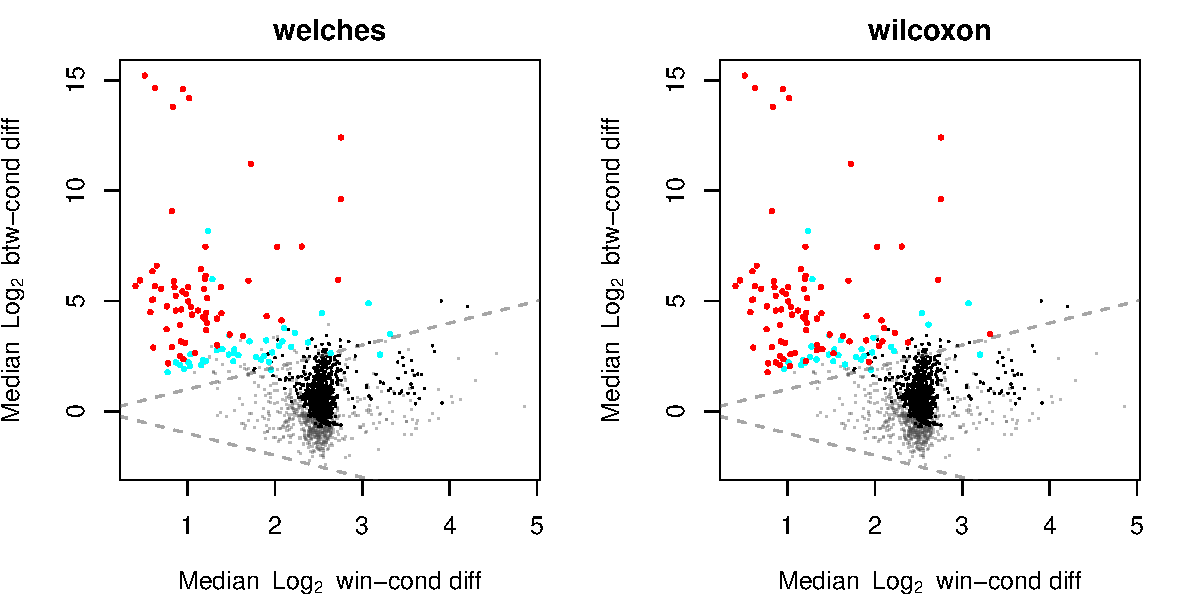
\includegraphics[width=6in]{/Users/ggloor/Documents/LaTeX/ALDEx/t-test_aldex/selex_mw.pdf}
\caption{Differential abundance in the selex dataset. The top row shows features called as significantly different using either Welches t-test, while the bottom rows shows the same for the Wilcoxon rank test. The left column shows q value false discovery rates (tail-area based method) and local false discovery method (density-based method). The false discovery rate was set at 0.1 in all cases. The diagonal dashed line represents equivalence between the within and between group variation. In this case, Welches t-test with a qval identified 106, and Wilcoxon with qval identified 90 differentially abundant variants, all of which were a subset of the variants identified by Welches t-test. }
\label{selex}
\end{center}
\end{figure}

\begin{verbatim}
library(ALDEx2)
#load the selex dataset
data(selex)
conds <- c("NS","NS","NS","NS","NS","NS","NS","S","S","S","S","S","S","S")

#run aldex
x <- aldex(selex, conds)

#summarize the results in a table
y <- summary.aldex(x) #now defaults to median TRUE

#plot the result to choose cutoff values
pdf("selex_mw.pdf")
par(mfrow=c(2,2), mar=c(4,4,2,2))
plot.aldex(x, test="welches", fdr="qval")
plot.aldex(x, test="welches", fdr="lfdr")
plot.aldex(x, test="wilcox", fdr="qval")
plot.aldex(x, test="wilcox", fdr="lfdr")
dev.off()
\end{verbatim}
\vspace{12pt}
In this instance,  shown in Figure \ref{selex}, it appears that the Welches or Wilcoxon tests with the tail-area based fdr (qval) is more informative. This is likely because these data are both very reproducible across all features due to a high number of read counts per feature and low biological variability (these are replicate growths of the same library) and because the number of features is less than in the previous example. We observe that when very small numbers of features are used, as would be the norm in a 16S rRNA sequencing experiment, that the q value correction is more powerful than the lfdr method.

 


%\begin{figure}[htbp]
%\begin{center}
%\includegraphics[width=4.5in]{/Users/ggloor/Documents/LaTeX/ALDEx/t-test_aldex/selex_hist.pdf}
%\caption{Histogram of p values in the Bottomly dataset. This dataset has low biological variability and the tail area-based q value would be a more powerful false discovery rate statistic in this instance.}
%\label{bottomly}
%\end{center}
%\end{figure}

\bibliography{bibdesk_refs}
\bibliographystyle{plos2009}




\end{document}  